\documentclass[11pt, a4paper]{article}
\usepackage[utf8]{inputenc}
\usepackage{amsmath, amssymb, amsthm}
\usepackage{graphicx}
\usepackage{geometry}
\usepackage{fancyhdr}
\usepackage{enumitem}
\usepackage{booktabs}
\usepackage{tikz}
\usepackage{xcolor}

% Page layout configuration
\geometry{left=2.5cm, right=2.5cm, top=2.5cm, bottom=2.5cm}
\pagestyle{fancy}
\fancyhf{}
\lhead{\textbf{Course:} Complex Systems Modeling}
\rhead{\textbf{Sample Solution}}
\lfoot{Department of Mechanical Engineering}
\rfoot{Page \thepage}

\title{\textbf{Sample Solution: Trial Exam}}
\author{Prof. Robert Flassig}
\date{}

\begin{document}

\maketitle

\section*{Problem 1: Fundamentals of Modeling (15 Points)}

\begin{enumerate}[label=\alph*)]
    \item \textbf{Box's Quote and Model Utility (5 pts)}
    \begin{itemize}
        \item \textbf{Explanation:} The quote "All models are wrong, but some are useful" highlights that every model is a simplified abstraction of reality and can never perfectly represent the infinite complexity of the real world. 
        \item \textbf{Useful vs. Correct:} A model does not need to be "correct" (perfectly true) to be valuable. It is considered "useful" if it helps us understand, predict, or control a system within a specific scope of applicability, despite its simplifications.
    \end{itemize}

    \item \textbf{Occam's Razor (5 pts)}
    \begin{itemize}
        \item \textbf{Definition:} Occam's Razor is the principle of simplicity. It suggests that among competing models with equal predictive power, one should choose the simpler one.
        \item \textbf{Application:} In modeling, this means eliminating unnecessary parameters and assumptions to focus on the core behavior, avoiding "overfitting".
    \end{itemize}

    \item \textbf{Validity vs. Robustness (5 pts)}
    \begin{itemize}
        \item \textbf{Validity:} Refers to how accurately a model's predictions match observed data and reality.
        \item \textbf{Robustness:} Refers to the stability of a model's predictions when its assumptions or parameter values are slightly varied. A robust model is trustworthy because it is not overly sensitive to minor errors or changes.
    \end{itemize}
\end{enumerate}

\section*{Problem 2: Scaling and Nondimensionalization (15 Points)}

\textbf{Given Equation:} $\frac{dx}{dt} = -r x \left(1 - \frac{x}{K}\right)$

\begin{enumerate}[label=\alph*)]
    \item \textbf{Substitution (5 pts)}
    We substitute the state variable and time with scaled dimensionless versions:
    $$ x = \alpha u, \quad t = \beta \tau $$
    Substituting these into the ODE:
    $$ \frac{d(\alpha u)}{d(\beta \tau)} = -r (\alpha u) \left(1 - \frac{\alpha u}{K}\right) $$
    $$ \frac{\alpha}{\beta} \frac{du}{d\tau} = -r \alpha u \left(1 - \frac{\alpha}{K} u\right) $$
    Dividing by $\frac{\alpha}{\beta}$:
    $$ \frac{du}{d\tau} = -r \beta u \left(1 - \frac{\alpha}{K} u\right) $$

    \item \textbf{Canonical Form (10 pts)}
    We want to eliminate parameters $r$ and $K$ by setting the coefficients to 1.
    \begin{enumerate}
        \item Set the coefficient of the linear term to 1:
        $$ r \beta = 1 \implies \beta = \frac{1}{r} $$
        \item Set the coefficient inside the parenthesis to 1:
        $$ \frac{\alpha}{K} = 1 \implies \alpha = K $$
    \end{enumerate}
    Substituting $\alpha$ and $\beta$ back into the equation:
    $$ \frac{du}{d\tau} = - (1) u (1 - 1 u) $$
    \textbf{Final dimensionless form:}
    $$ \frac{du}{d\tau} = -u(1-u) \quad \text{or} \quad \frac{du}{d\tau} = u^2 - u $$
    \textit{(Note: Standard logistic growth typically uses $+r$, which results in $u(1-u)$. Based on the specific equation in the exam with $-r$, the result is $-u(1-u)$.)}.
\end{enumerate}

\section*{Problem 3: Linear Dynamical Systems (20 Points)}

\textbf{System Matrix:} $\mathbf{A} = \begin{pmatrix} 0 & 1 \\ -4 & -2 \end{pmatrix}$

\begin{enumerate}[label=\alph*)]
    \item \textbf{Trace and Determinant (5 pts)}
    \begin{itemize}
        \item Trace: $\text{Tr}(\mathbf{A}) = a + d = 0 + (-2) = -2$.
        \item Determinant: $\det(\mathbf{A}) = ad - bc = (0)(-2) - (1)(-4) = 4$.
    \end{itemize}

    \item \textbf{Eigenvalues and Stability (10 pts)}
    The characteristic equation is $\lambda^2 - \text{Tr}(\mathbf{A})\lambda + \det(\mathbf{A}) = 0$:
    $$ \lambda^2 - (-2)\lambda + 4 = 0 \implies \lambda^2 + 2\lambda + 4 = 0 $$
    Solving for $\lambda$:
    $$ \lambda_{1,2} = \frac{-2 \pm \sqrt{2^2 - 4(1)(4)}}{2} = \frac{-2 \pm \sqrt{4 - 16}}{2} = \frac{-2 \pm \sqrt{-12}}{2} $$
    $$ \lambda_{1,2} = -1 \pm i\sqrt{3} $$
    \textbf{Classification:}
    \begin{itemize}
        \item The real part is negative ($\text{Re}(\lambda) = -1 < 0$).
        \item The eigenvalues are complex conjugates ($\text{Im}(\lambda) \neq 0$).
        \item Therefore, the origin is a \textbf{Stable Spiral} (or Spiral Sink).
    \end{itemize}

    \item \textbf{Physical Interpretation (5 pts)}
    Comparing the characteristic equation $\lambda^2 + 2\lambda + 4 = 0$ to the mass-spring-damper standard form $s^2 + 2\zeta\omega_n s + \omega_n^2 = 0$:
    \begin{itemize}
        \item Natural frequency $\omega_n^2 = 4 \implies \omega_n = 2$.
        \item Damping term $2\zeta\omega_n = 2 \implies 2\zeta(2) = 2 \implies \zeta = 0.5$.
    \end{itemize}
    Since the damping ratio $\zeta < 1$ (and eigenvalues are complex), the system is \textbf{Underdamped}.
\end{enumerate}

\section*{Problem 4: Bifurcation Analysis (20 Points)}

\textbf{System:} $\dot{x} = \mu x - x^3 = x(\mu - x^2)$

\begin{enumerate}[label=\alph*)]
    \item \textbf{Fixed Points (5 pts)}
    Set $\dot{x} = 0$:
    $$ x(\mu - x^2) = 0 $$
    This gives $x^* = 0$ always.
    \begin{itemize}
        \item If $\mu < 0$: $\mu - x^2 = 0$ has no real solutions. Only fixed point is $x^* = 0$.
        \item If $\mu > 0$: $\mu - x^2 = 0 \implies x^2 = \mu \implies x^* = \pm\sqrt{\mu}$. Three fixed points: $0, +\sqrt{\mu}, -\sqrt{\mu}$.
    \end{itemize}

    \item \textbf{Linear Stability (5 pts)}
    Jacobian $f'(x) = \frac{d}{dx}(\mu x - x^3) = \mu - 3x^2$.
    Evaluate at the origin $x^* = 0$:
    $$ f'(0) = \mu $$
    \begin{itemize}
        \item If $\mu < 0$: $f'(0) < 0 \implies$ \textbf{Stable}.
        \item If $\mu > 0$: $f'(0) > 0 \implies$ \textbf{Unstable}.
    \end{itemize}

    \item \textbf{Bifurcation Type (5 pts)}
    At $\mu=0$, the stable fixed point at the origin becomes unstable, and two new stable fixed points appear ($\pm\sqrt{\mu}$).
    This is a \textbf{Supercritical Pitchfork Bifurcation}.

    \item \textbf{Sketch (5 pts)}
    \begin{center}
    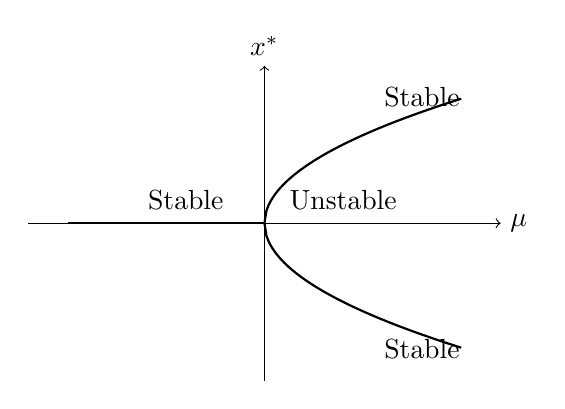
\begin{tikzpicture}
        \draw[->] (-3,0) -- (3,0) node[right] {$\mu$};
        \draw[->] (0,-2) -- (0,2) node[above] {$x^*$};
        % Stable branch for mu < 0 (x=0)
        \draw[thick] (-2.5,0) -- (0,0);
        % Unstable branch for mu > 0 (x=0)
        \draw[dashed] (0,0) -- (2.5,0);
        % Stable branches for mu > 0 (parabola)
        \draw[thick, domain=0:2.5, samples=100] plot (\x, {sqrt(\x)});
        \draw[thick, domain=0:2.5, samples=100] plot (\x, {-sqrt(\x)});
        \node at (2, 1.6) {Stable};
        \node at (2, -1.6) {Stable};
        \node at (-1, 0.3) {Stable};
        \node at (1, 0.3) {Unstable};
    \end{tikzpicture}
    \end{center}
\end{enumerate}

\section*{Problem 5: Phase Space Reconstruction (20 Points)}

\textbf{System:} $\dot{x} = y, \quad \dot{y} = xy - x^2 = x(y-x)$

\begin{enumerate}[label=\alph*)]
    \item \textbf{Nullclines (5 pts)}
    \begin{itemize}
        \item $\dot{x}$-nullcline: Set $\dot{x} = 0 \implies y = 0$. (This is the x-axis).
        \item $\dot{y}$-nullcline: Set $\dot{y} = 0 \implies x(y-x) = 0$. This gives two lines: $x = 0$ (y-axis) and $y = x$ (diagonal).
    \end{itemize}

    \item \textbf{Fixed Points (5 pts)}
    Intersection of $\dot{x}=0$ and $\dot{y}=0$:
    $$ y=0 \quad \text{AND} \quad (x=0 \text{ or } y=x) $$
    If $y=0$ and $x=0$, point is $(0,0)$.
    If $y=0$ and $y=x$, point is $(0,0)$.
    Unique Fixed Point: \textbf{(0,0)}.

    \item \textbf{Sketch and Directions (10 pts)}
    Regions defined by lines $y=0$, $x=0$, $y=x$.
    \begin{itemize}
        \item \textbf{Region I ($x>0, y>x$):} Let $x=1, y=2$. $\dot{x}=2 (>0)$, $\dot{y}=1(2-1)=1 (>0)$. Direction $\nearrow$ (North-East).
        \item \textbf{Region II ($x>0, 0<y<x$):} Let $x=2, y=1$. $\dot{x}=1 (>0)$, $\dot{y}=2(1-2)=-2 (<0)$. Direction $\searrow$ (South-East).
        \item \textbf{Region III ($x>0, y<0$):} Let $x=1, y=-1$. $\dot{x}=-1 (<0)$, $\dot{y}=1(-1-1)=-2 (<0)$. Direction $\swarrow$ (South-West).
        \item \textbf{Region IV ($x<0, y>0$):} Let $x=-1, y=1$. $\dot{x}=1 (>0)$, $\dot{y}=-1(1-(-1))=-2 (<0)$. Direction $\searrow$ (South-East).
    \end{itemize}
    
    \begin{center}
    \begin{tikzpicture}
        \draw[->] (-3,0) -- (3,0) node[right] {$x$};
        \draw[->] (0,-3) -- (0,3) node[above] {$y$};
        
        % Nullclines
        \draw[blue, thick] (-3,0) -- (3,0) node[below right] {$\dot{x}=0$};
        \draw[red, thick] (0,-3) -- (0,3) node[right] {$\dot{y}=0$};
        \draw[red, thick] (-3,-3) -- (3,3) node[right] {$\dot{y}=0$};
        
        % Fixed point
        \filldraw [black] (0,0) circle (2pt);
        
        % Arrows
        \draw[->, thick] (0.5, 1.5) -- (1, 2); % Region I
        \draw[->, thick] (2, 1) -- (2.5, 0.5); % Region II
        \draw[->, thick] (1, -1) -- (0.5, -2); % Region III
        \draw[->, thick] (-1, 1) -- (-0.5, 0.5); % Region IV
    \end{tikzpicture}
    \end{center}
\end{enumerate}

\section*{Problem 6: Chaos Theory (10 Points)}

\begin{enumerate}[label=\alph*)]
    \item \textbf{Definition (5 pts)}
    Chaos is the long-term aperiodic behavior in a deterministic system that exhibits sensitivity to initial conditions. Sensitivity means that two trajectories starting arbitrarily close together will diverge exponentially fast, making long-term prediction impossible (Butterfly Effect).

    \item \textbf{Lyapunov Exponent (5 pts)}
    The Lyapunov exponent $\lambda$ measures the average rate of divergence of nearby trajectories.
    \begin{itemize}
        \item If $\lambda > 0$, the trajectories diverge exponentially, implying the system is \textbf{Chaotic} and unpredictable in the long run.
    \end{itemize}
\end{enumerate}

\section*{Bonus Question: Continuous-Time Chaos (+5 Points)}

\textbf{Answer:} No, chaos cannot exist in a continuous-time system with only 2 state variables.
\textbf{Reasoning:} According to the \textbf{Poincaré-Bendixson theorem}, trajectories in a 2D continuous phase space cannot cross each other. Since chaos requires the "stretching and folding" of trajectories (mixing) while remaining bounded, this geometry is topologically impossible in 2D without intersection. Chaos requires at least \textbf{3 dimensions} in continuous systems (e.g., the Lorenz system).

\end{document}